\documentclass[11pt,a4paper]{report}
\usepackage{fullpage}
\usepackage{listings}
\usepackage{graphicx}
\usepackage[usenames,dvipsnames]{color}
% This is the color used for MATLAB comments below
\definecolor{MyDarkGreen}{rgb}{0.0,0.4,0.0}
 
% For faster processing, load Matlab syntax for listings
\lstloadlanguages{Matlab}%
\lstset{language=Matlab,                        % Use MATLAB
        frame=single,                           % Single frame around code
        basicstyle=\scriptsize\sffamily,             % Use small true type font
        keywordstyle=[1]\color{Blue}\bfseries,        % MATLAB functions bold and blue
        keywordstyle=[2]\color{Purple},         % MATLAB function arguments purple
        keywordstyle=[3]\color{Blue}\underbar,  % User functions underlined and blue
        identifierstyle=,                       % Nothing special about identifiers
                                                % Comments small dark green courier
        commentstyle=\usefont{T1}{pcr}{m}{sl}\color{MyDarkGreen}\scriptsize,
        stringstyle=\color{Purple},             % Strings are purple
        showstringspaces=false,                 % Don't put marks in string spaces
        tabsize=5,                              % 5 spaces per tab
        %
        %%% Put standard MATLAB functions not included in the default
        %%% language here
        morekeywords={xlim,ylim,var,alpha,factorial,poissrnd,normpdf,normcdf},
        %
        %%% Put MATLAB function parameters here
        morekeywords=[2]{on, off, interp},
        %
        %%% Put user defined functions here
        morekeywords=[3]{FindESS, homework_example},
        %
        morecomment=[l][\color{Blue}]{...},     % Line continuation (...) like blue comment
        numbers=left,                           % Line numbers on left
        firstnumber=1,                          % Line numbers start with line 1
        numberstyle=\tiny\color{Blue},          % Line numbers are blue
        stepnumber=5                            % Line numbers go in steps of 5
        }

\begin{document}


\begin{center}
{\large Homework 1: Giri Subramanian}
\end{center}

The code is given below. \\
Problem 1: \lstinputlisting{Giri_Subramanian_1.m} 


The plots generated have been attached below.

\begin{center}
\begin{figure}[!ht]
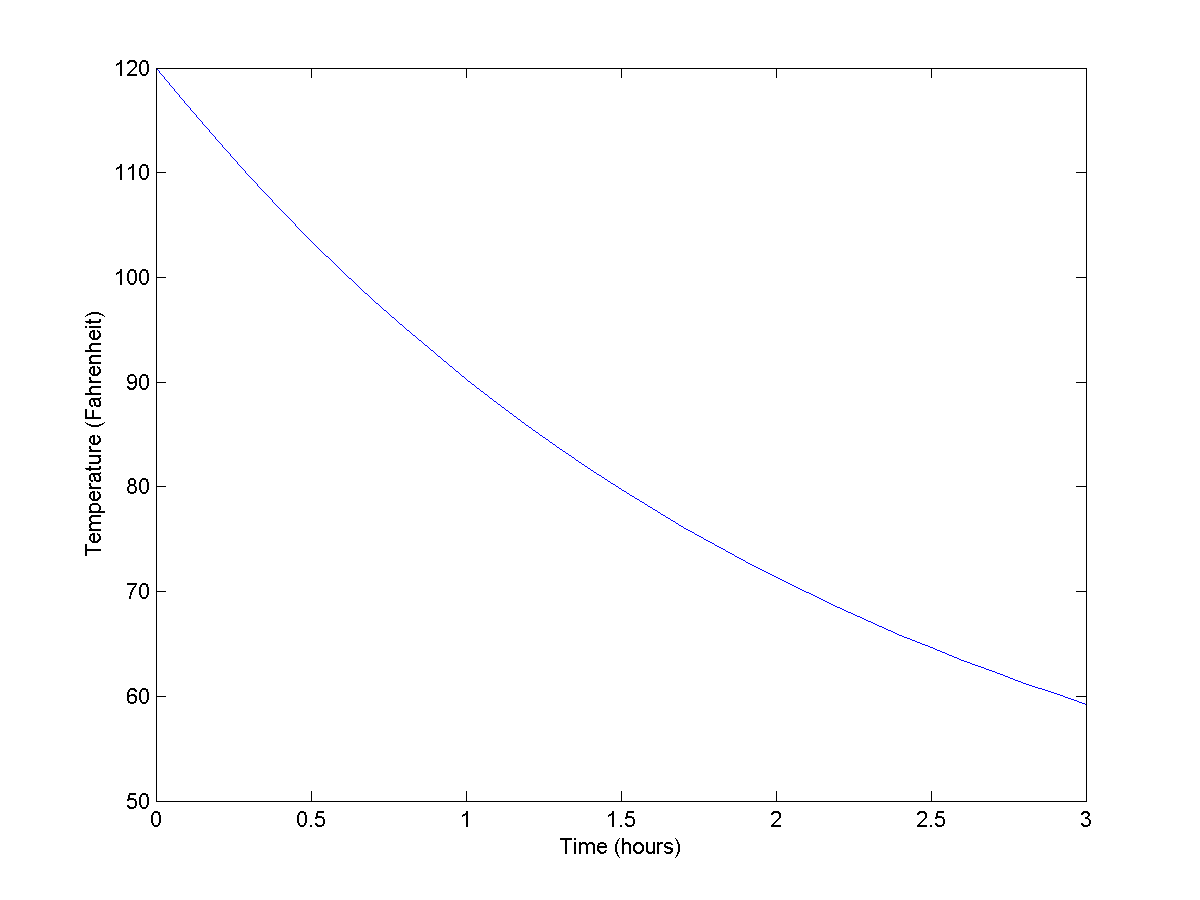
\includegraphics[scale=0.75]{Giri_Subramanian_HW_1_Problem_1}
\caption{Question 1}
\end{figure}

\begin{figure}[!ht]
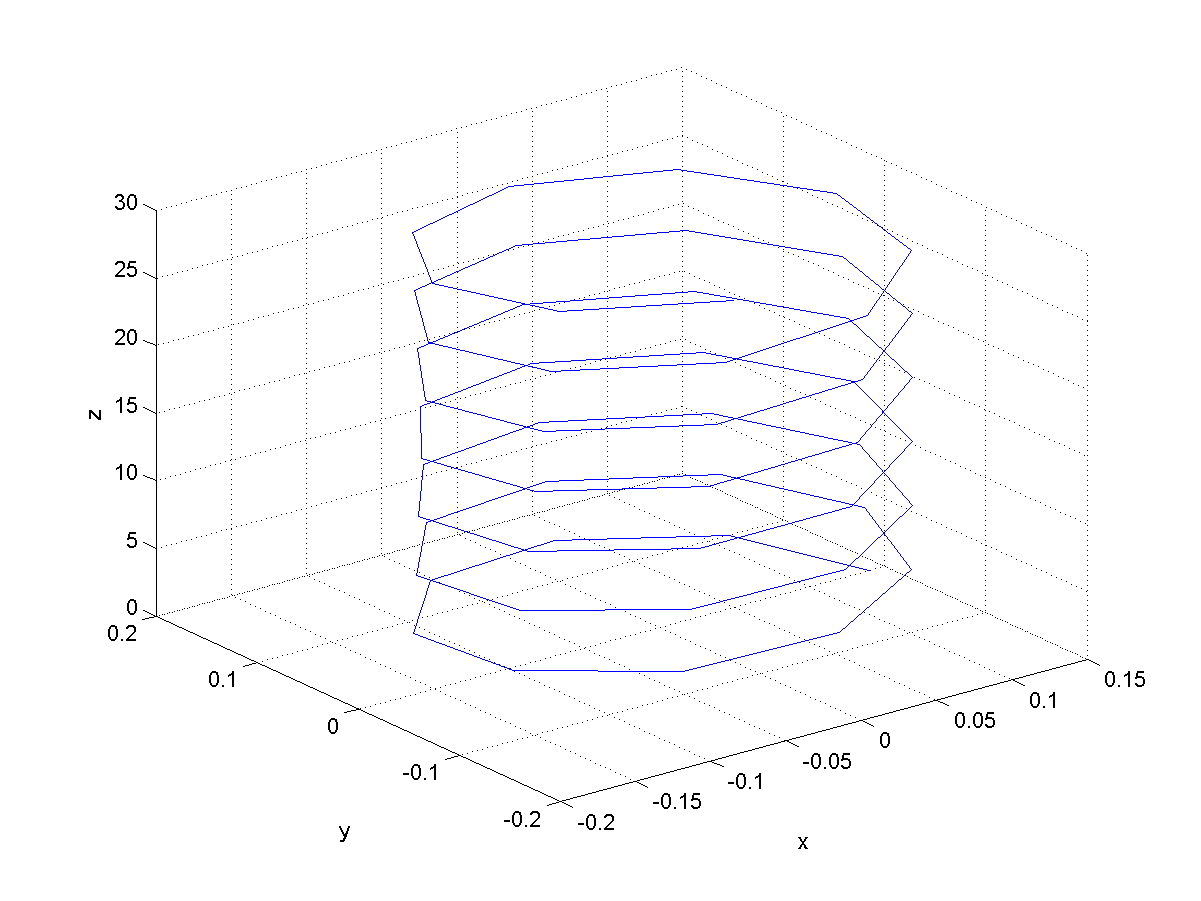
\includegraphics[scale=0.75]{Giri_Subramanian_HW_1_Problem_2a}
\caption{Question 2}
\end{figure}
\end{center}

\begin{center}
\begin{figure}[!h]
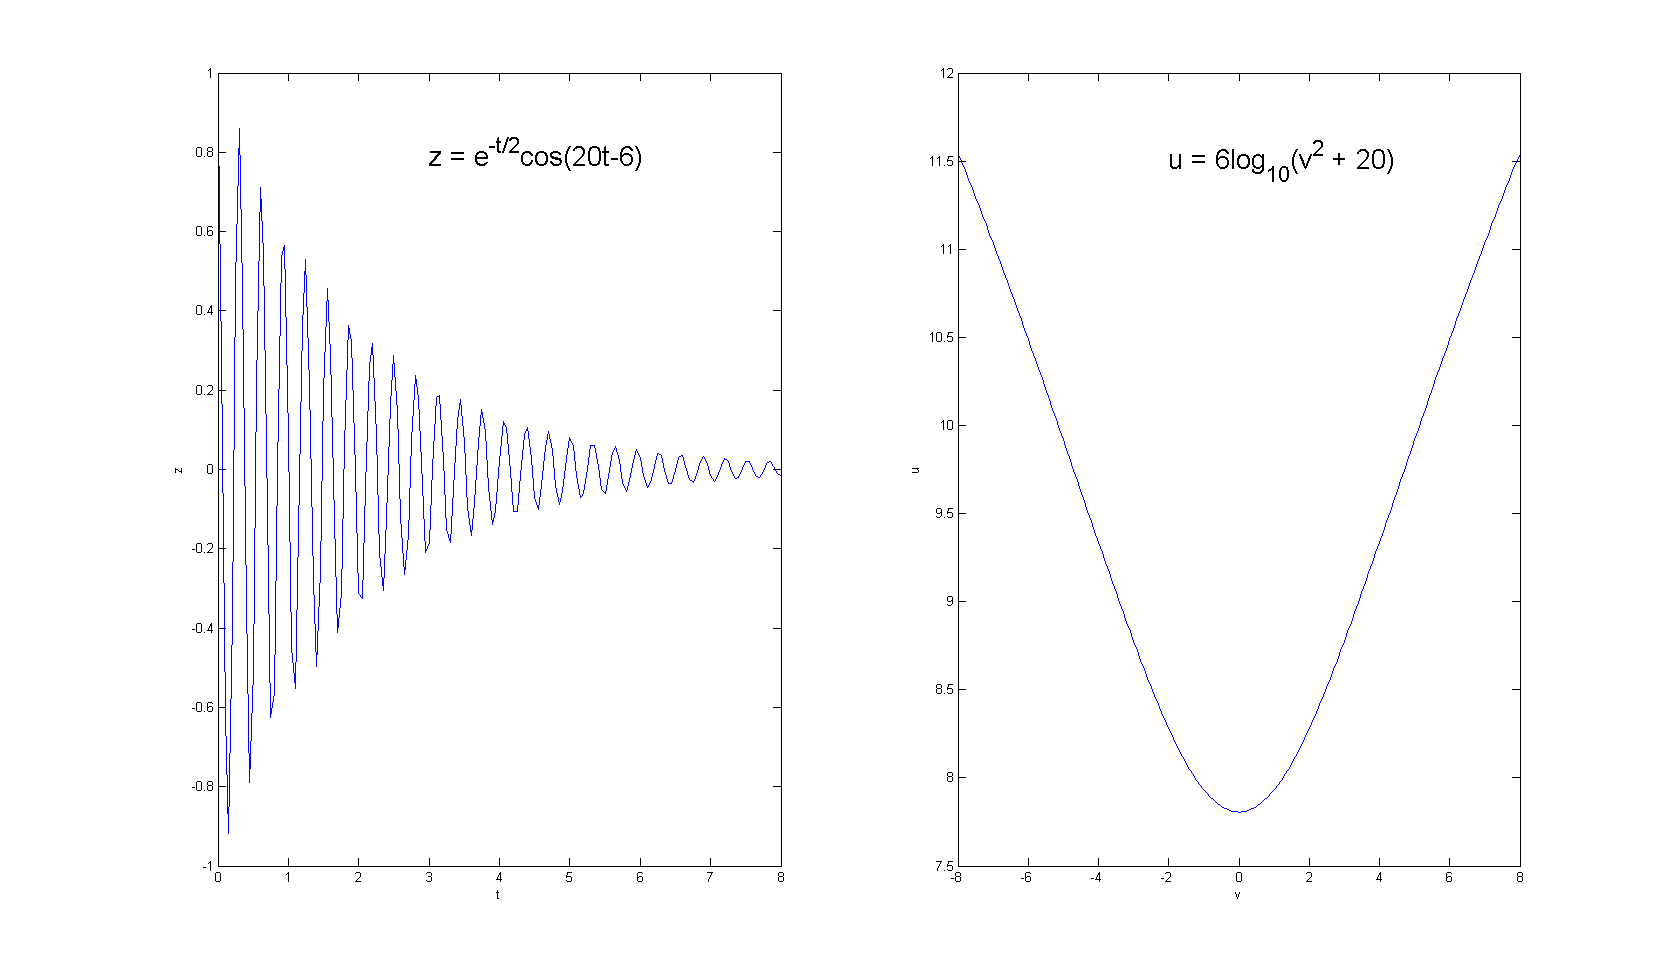
\includegraphics[scale=0.4]{Giri_Subramanian_HW_1_Problem_3}
\caption{Question 3}
\end{figure}

\begin{figure}[!h]
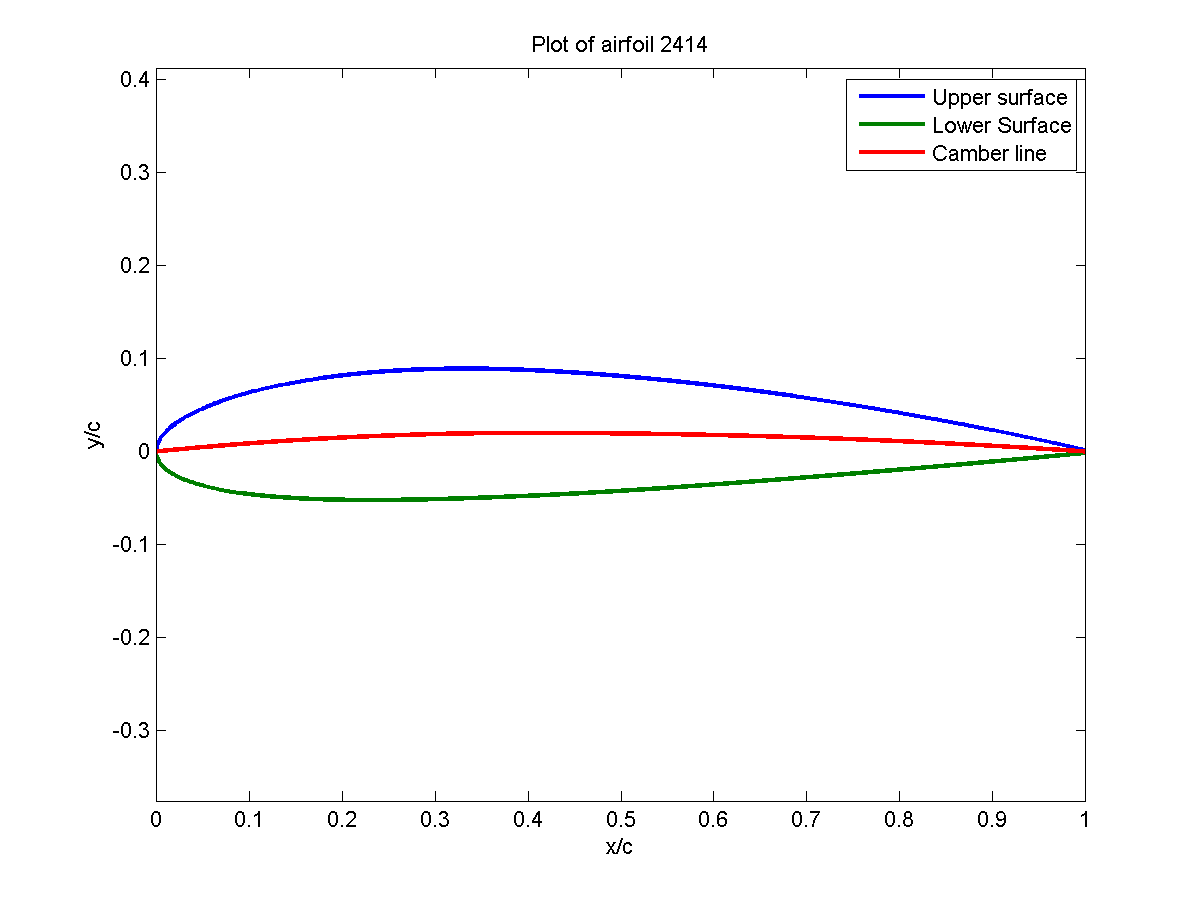
\includegraphics[scale=0.75]{Giri_Subramanian_HW_1_Problem_4}
\caption{Question 4}
\end{figure}
\end{center}



\end{document}